
\appendix

\chapter{Uitgebreide weergave van sub-experiment Term weighting}\label{bijlage term}

%tabel klein experiment term weighting 
\begin{table}
\centering
\begin{tabu} to \textwidth {|X|X|}
\hline
{\bf Recensie}                                                                                                                                                                                                                                                                                                                                                                                                                                                                                                                                                                                                                                                                                                                                                                                                                                                                                                                                                                                                                                                                                                                                                                                                                                                                                                                                                                                                                                                                                  & {\bf Woord met hoogste tf-idf score} \\ \hline
in het begin dacht ik echt van.. wat is dit nou weer.. maar je wil hem PERSE afzien! kei mooie film!aanrader!                                                                                                                                                                                                                                                                                                                                                                                                                                                                                                                                                                                                                                                                                                                                                                                                                                                                                                                                                                                                                                                                                                                                                                                                                                                                                                                                                                                   & Kei                                  \\ \hline
Geweldig verhaal! Aangrijpend. Ik heb deze film een stuk of 4 keer gezien, blijft indrukwekkend.****-sterren                                                                                                                                                                                                                                                                                                                                                                                                                                                                                                                                                                                                                                                                                                                                                                                                                                                                                                                                                                                                                                                                                                                                                                                                                                                                                                                                                                                    & Aangrijpend                          \\ \hline
Wat een geweldige film. De trilogy al 100 x gezien en het blijft goed. Ook vooral als je een de filosofie erachter zoekt zit er zoooooo veel meer achter dan mensen denken.Als je denkt dat dit zomaar een actiefilm scy fi met een paar moeilijke zinnen is zit je grandioos verkeerd. Dat is geen mening maar een simpel feit.Als je wat onderzoek ernaar doet zul je zien waar de personen hun namen aan te danken hebben en dat zelfs het kamernummer van Mr.Anderson (neo) een anagram/puzzel is. Dit gaat 10x zo diep als bijvoorbeeld The Da Vinci code ooit maar geprobeerd heeft te halen.                                                                                                                                                                                                                                                                                                                                                                                                                                                                                                                                                                                                                                                                                                                                                                                                                                                                                             & Je                                   \\ \hline
Coole film!                                                                                                                                                                                                                                                                                                                                                                                                                                                                                                                                                                                                                                                                                                                                                                                                                                                                                                                                                                                                                                                                                                                                                                                                                                                                                                                                                                                                                                                                                     & Coole                                \\ \hline
Voor mij een 5 sterren film. Ik had hem op dezelfde manier gemaakt. Inspirerende film                                                                                                                                                                                                                                                                                                                                                                                                                                                                                                                                                                                                                                                                                                                                                                                                                                                                                                                                                                                                                                                                                                                                                                                                                                                                                                                                                                                                           & Inspirerende                         \\ \hline
Geweldige nagelbijtende oorlogsfilm,zo zie je ze jammer genoeg zelden,zien !!!!                                                                                                                                                                                                                                                                                                                                                                                                                                                                                                                                                                                                                                                                                                                                                                                                                                                                                                                                                                                                                                                                                                                                                                                                                                                                                                                                                                                                                 & nagelbijtende                        \\ \hline
Een prachtige en zeer meeslepende film. Het blijft ook erg boeiend, omdat je veel verschillende dingen te zien krijgt. De beelden van de oorlog waren soms echt verschrikkelijk om te zien, maar zo ging het er wel aan toe en dus kwam het zeer geloofwaardig over. Omdat de afwisseling best groot is gaat het nergens echt vervelen. Je hebt momenten waar er volop actie is en het ook best spannend is wat er gaat gebeuren, maar er zijn ook de nodige rustige momenten waar goed de tijd wordt genomen om de personages beter te leren kennen.Leonardo DiCaprio zet wel echt een hele sterke rol neer. We wisten allemaal al dat het een goede acteur is, maar soms vind ik hem wat te wisselvallig. Daar is in deze film geen sprake van. Erg sterk gedaan. Ook Djimon Hounsou doet het heel goed als vader die er alles aan doet om zijn zoon te redden. Jennifer Connelly is een prettige verschijning, maar door haar komst werd er toch weer een beetje een liefdesverhaaltje in het verhaal gepropt. Dat had van mij niet gehoeven, al begrijp ik het wel.Wat misschien nog wel het beste aan deze film is zijn de waanzinnig mooie locaties. Ik heb genoten van bijna ieder shot. Vooral toen er uitgezoomd werd en je het hele landschap kon zien. Daar is veel aandacht aan besteed en de uitwerking is wat mij betreft fenomenaal. Het einde had ook nog best iets verrassends en dat maakt het een heel mooi geheel. 4,5* voor nu, wellicht na een herziening de volle score. & het                                  \\ \hline
Ik vind dat dit een overgewardeerde film is, net als een heleboel andere Nederlandse films op deze site.                                                                                                                                                                                                                                                                                                                                                                                                                                                                                                                                                                                                                                                                                                                                                                                                                                                                                                                                                                                                                                                                                                                                                                                                                                                                                                                                                                                        & overgewardeerde                      \\ \hline
\end{tabu}
\end{table}



\chapter{Resultaten Engelse gevoelsanalyse versus Nederlandse gevoelsanalyse}\label{bijlage vs}

\begin{table}
\centering
\caption{Resultaten Engelse gevoelsanalyse met de Decision Tree}
\begin{adjustbox}{width=1\textwidth}
\begin{tabular}{|l|l|l|l|l|l|l|}
\hline
{\bf Nr} & {\bf Title}                                                                      & {\bf Precisie trainingsset} & {\bf Precisie testset} & {\bf OG BI($\alpha=0,05$)} & {\bf BG BI ($\alpha=0,05$)} & {\bf $\sigma$} \\ \hline
1        & Bag of Words                                                                     & 70,96\%                     & 69,06\%                & 68,56\%                 & 69,56\%                  & 1,31\%      \\ \hline
2        & Best Feature selection + Bag of Words                                            & 69,84\%                     & 69,43\%                & 69,05\%                 & 69,80\%                  & 0,98\%      \\ \hline
3        & Best Feature selection + Term Weighting                                          & 71,09\%                     & 69,79\%                & 69,39\%                 & 70,19\%                  & 1,06\%      \\ \hline
4        & Bigrams                                                                          & 70,89\%                     & 69,41\%                & 69,02\%                 & 69,80\%                  & 1,02\%      \\ \hline
5        & LSA + Bag of Words                                                               & 67,71\%                     & 62,07\%                & 61,42\%                 & 62,71\%                  & 1,70\%      \\ \hline
6        & LSA + Term Weighting                                                             & 75,52\%                     & 71,54\%                & 71,12\%                 & 71,95\%                  & 1,09\%      \\ \hline
7        & Term Weighting                                                                   & 71,53\%                     & 69,76\%                & 69,34\%                 & 70,18\%                  & 1,11\%      \\ \hline
8        & Term weighting  + Bigrams                                                        & 71,74\%                     & 69,28\%                & 68,92\%                 & 69,64\%                  & 0,94\%      \\ \hline
9        & Verwijderen van stopwoorden                                                      & 70,80\%                     & 69,45\%                & 69,10\%                 & 69,80\%                  & 0,92\%      \\ \hline
10       & Verwijderen van stopwoorden + Best feature selection + Bag of Words   & 70,45\%                     & 69,36\%                & 68,85\%                 & 69,86\%                  & 1,33\%      \\ \hline
11       & Verwijderen van stopwoorden + Best feature selection + Term Weighting & 71,14\%                     & 69,47\%                & 68,97\%                 & 69,97\%                  & 1,30\%      \\ \hline
12       & Verwijderen van stopwoorden + Bigrams                                            & 70,85\%                     & 69,51\%                & 69,15\%                 & 69,87\%                  & 0,95\%      \\ \hline
13       & Verwijderen van stopwoorden + Bigrams + Term Weighting                           & 71,37\%                     & 69,44\%                & 69,08\%                 & 69,80\%                  & 0,94\%      \\ \hline
14       & Verwijderen van stopwoorden + LSA + Bag of Words                                 & 72,96\%                     & 68,66\%                & 68,07\%                 & 69,25\%                  & 1,55\%      \\ \hline
15       & Verwijderen van stopwoorden + LSA + Term Weighting                               & 79,21\%                     & 75,50\%                & 75,05\%                 & 75,95\%                  & 1,18\%      \\ \hline
16       & Verwijderen van stopwoorden + Term Weighting                                     & 71,40\%                     & 69,60\%                & 69,20\%                 & 70,00\%                  & 1,06\%      \\ \hline
\end{tabular}
\end{adjustbox}
\end{table}



\begin{table}
\centering
\caption{Resultaten Engelse gevoelsanalyse met de Naive Bayes Classifier}
\begin{adjustbox}{width=1\textwidth}
\begin{tabular}{|l|l|l|l|l|l|l|}
\hline
{\bf Nr} & {\bf Title}                                                                      & {\bf Precisie trainingsset} & {\bf Precisie testset} & {\bf OG BI($\alpha=0,05$)} & {\bf BG BI ($\alpha=0,05$)} & {\bf $\sigma$} \\ \hline
1        & Bag of Words                                                                     & 94,25\%                     & 85,74\%                & 85,39\%                 & 86,10\%                  & 0,93\%      \\ \hline
2        & Best Feature selection + Bag of Words                                            & 75,21\%                     & 74,90\%                & 74,55\%                 & 75,24\%                  & 0,90\%      \\ \hline
3        & Best Feature selection + Term Weighting                                          & 67,98\%                     & 67,79\%                & 67,31\%                 & 68,26\%                  & 1,25\%      \\ \hline
4        & Bigrams                                                                          & 99,82\%                     & 89,23\%                & 88,94\%                 & 89,52\%                  & 0,76\%      \\ \hline
5        & LSA + Bag of Words                                                               & 63,97\%                     & 63,11\%                & 61,08\%                 & 65,14\%                  & 0,53\%      \\ \hline
6        & LSA + Term Weighting                                                             & 80,45\%                     & 78,98\%                & 78,20\%                 & 79,77\%                  & 2,06\%      \\ \hline
7        & Term Weighting                                                                   & 94,42\%                     & 86,75\%                & 86,44\%                 & 87,06\%                  & 0,82\%      \\ \hline
8        & Term weighting  + Bigrams                                                        & 99,14\%                     & 89,00\%                & 88,71\%                 & 89,28\%                  & 0,75\%      \\ \hline
9        & Verwijderen van stopwoorden                                                      & 95,39\%                     & 86,62\%                & 86,33\%                 & 86,92\%                  & 0,78\%      \\ \hline
10       & Verwijderen van stopwoorden + Best feature selection + Bag of Words   & 74,98\%                     & 74,43\%                & 74,13\%                 & 74,73\%                  & 0,80\%      \\ \hline
11       & Verwijderen van stopwoorden + Best feature selection + Term Weighting & 75,18\%                     & 74,94\%                & 74,59\%                 & 75,29\%                  & 0,92\%      \\ \hline
12       & Verwijderen van stopwoorden + Bigrams                                            & 99,96\%                     & 89,23\%                & 88,94\%                 & 89,52\%                  & 0,76\%      \\ \hline
13       & Verwijderen van stopwoorden + Bigrams + Term Weighting                           & 99,23\%                     & 89,29\%                & 88,95\%                 & 89,63\%                  & 0,90\%      \\ \hline
14       & Verwijderen van stopwoorden + LSA + Bag of Words                                 & 55,16\%                     & 54,88\%                & 54,33\%                 & 55,43\%                  & 1,45\%      \\ \hline
15       & Verwijderen van stopwoorden + LSA + Term Weighting                               & 76,87\%                     & 73,58\%                & 71,31\%                 & 75,85\%                  & 5,97\%      \\ \hline
16       & Verwijderen van stopwoorden + Term Weighting                                     & 95,35\%                     & 87,41\%                & 87,14\%                 & 87,68\%                  & 0,70\%      \\ \hline
\end{tabular}
\end{adjustbox}
\end{table}

\begin{table}
\centering
\caption{Resultaten Nederlandse gevoelsanalyse met de Decision Tree}
\begin{adjustbox}{width=1\textwidth}
\begin{tabular}{|l|l|l|l|l|l|l|}
\hline
{\bf Nr} & {\bf Title}                                                                      & {\bf Precisie trainingsset} & {\bf Precisie testset} & {\bf OG BI($\alpha=0,05$)} & {\bf BG BI ($\alpha=0,05$)} & {\bf $\sigma$} \\ \hline
1        & Bag of Words                                                                     & 61,00\%                     & 59,34\%                & 58,86\%                 & 59,82\%                  & 1,26\%      \\ \hline
2        & Best Feature selection + Term Weighting                                          & 61,16\%                     & 59,35\%                & 58,87\%                 & 59,82\%                  & 1,25\%      \\ \hline
3        & Best Feature selection Bag of Words                                              & 60,88\%                     & 59,45\%                & 58,96\%                 & 59,94\%                  & 1,30\%      \\ \hline
4        & Bigrams                                                                          & 61,54\%                     & 59,35\%                & 58,85\%                 & 59,86\%                  & 1,32\%      \\ \hline
5        & LSA + Bag of Words                                                               & 63,03\%                     & 57,53\%                & 57,01\%                 & 58,05\%                  & 1,37\%      \\ \hline
6        & LSA + Term Weighting                                                             & 64,48\%                     & 58,58\%                & 58,09\%                 & 59,07\%                  & 1,28\%      \\ \hline
7        & Term Weighting                                                                   & 61,68\%                     & 58,83\%                & 58,30\%                 & 59,35\%                  & 1,38\%      \\ \hline
8        & Term weighting  + Bigrams                                                        & 61,72\%                     & 59,06\%                & 58,56\%                 & 59,56\%                  & 1,31\%      \\ \hline
9        & Verwijderen van stopwoorden                                                      & 58,45\%                     & 56,82\%                & 56,21\%                 & 57,43\%                  & 1,62\%      \\ \hline
10       & Verwijderen van stopwoorden + Best feature selection + Bag of Words   & 57,88\%                     & 56,74\%                & 56,25\%                 & 57,24\%                  & 1,30\%      \\ \hline
11       & Verwijderen van stopwoorden + Best feature selection + Term Weighting & 57,84\%                     & 56,44\%                & 55,90\%                 & 56,97\%                  & 1,41\%      \\ \hline
12       & Verwijderen van stopwoorden + Bigrams                                            & 58,44\%                     & 56,80\%                & 56,20\%                 & 74,12\%                  & 1,60\%      \\ \hline
13       & Verwijderen van stopwoorden + Bigrams + Term Weighting                           & 58,68\%                     & 56,58\%                & 55,95\%                 & 57,21\%                  & 1,65\%      \\ \hline
14       & Verwijderen van stopwoorden + LSA + Bag of Words                                 & 62,89\%                     & 57,23\%                & 56,74\%                 & 57,71\%                  & 1,27\%      \\ \hline
15       & Verwijderen van stopwoorden + LSA + Term Weighting                               & 64,59\%                     & 59,24\%                & 58,75\%                 & 59,72\%                  & 1,18\%      \\ \hline
16       & Verwijderen van stopwoorden + Term Weighting                                     & 58,68\%                     & 56,55\%                & 55,91\%                 & 57,19\%                  & 1,68\%      \\ \hline
\end{tabular}
\end{adjustbox}
\end{table}

\begin{table}
\centering
\caption{Resultaten Nederlandse gevoelsanalyse met de Naive Bayes Classifier}
\begin{adjustbox}{width=1\textwidth}
\begin{tabular}{|l|l|l|l|l|l|l|}
\hline
{\bf Nr} & {\bf Title}                                                                      & {\bf Precisie trainingsset} & {\bf Precisie testset} & {\bf OG BI($\alpha=0,05$)} & {\bf BG BI ($\alpha=0,05$)} & {\bf $\sigma$} \\ \hline
1        & Bag of Words                                                                     & 88,83\%                     & 70,51\%                & 70,09\%                 & 70,92\%                  & 1,09\%      \\ \hline
2        & Best Feature selection + Bag of Words                                            & 60,41\%                     & 59,53\%                & 58,85\%                 & 60,21\%                  & 1,78\%      \\ \hline
3        & Best Feature selection + Term Weighting                                          & 59,02\%                     & 58,86\%                & 58,14\%                 & 59,59\%                  & 1,90\%      \\ \hline
4        & Bigrams                                                                          & 97,96\%                     & 70,20\%                & 69,77\%                 & 70,63\%                  & 1,13\%      \\ \hline
5        & LSA + Bag of Words                                                               & 54,86\%                     & 54,84\%                & 54,51\%                 & 55,16\%                  & 0,87\%      \\ \hline
6        & LSA + Term Weighting                                                             & 65,07\%                     & 63,15\%                & 62,49\%                 & 63,81\%                  & 1,74\%      \\ \hline
7        & Term Weighting                                                                   & 87,93\%                     & 69,40\%                & 69,04\%                 & 69,76\%                  & 0,94\%      \\ \hline
8        & Term weighting  + Bigrams                                                        & 95,41\%                     & 67,96\%                & 67,54\%                 & 68,38\%                  &             \\ \hline
9        & Verwijderen van stopwoorden                                                      & 89,88\%                     & 70,35\%                & 69,96\%                 & 70,74\%                  & 1,03\%      \\ \hline
10       & Verwijderen van stopwoorden + Best feature selection + Bag of Words   & 60,32\%                     & 59,18\%                & 58,62\%                 & 59,73\%                  & 1,46\%      \\ \hline
11       & Verwijderen van stopwoorden + Best feature selection + Term Weighting & 61,61\%                     & 60,76\%                & 59,88\%                 & 61,63\%                  & 2,30\%      \\ \hline
12       & Verwijderen van stopwoorden + Bigrams                                            & 98,47\%                     & 70,63\%                & 70,26\%                 & 71,00\%                  & 0,98\%      \\ \hline
13       & Verwijderen van stopwoorden + Bigrams + Term Weighting                           & 98,71\%                     & 70,66\%                & 70,30\%                 & 71,01\%                  & 0,93\%      \\ \hline
14       & Verwijderen van stopwoorden + LSA + Bag of Words                                 & 54,35\%                     & 53,74\%                & 53,41\%                 & 54,07\%                  & 0,87\%      \\ \hline
15       & Verwijderen van stopwoorden + LSA + Term Weighting                               & 61,59\%                     & 60,15\%                & 59,64\%                 & 60,65\%                  & 1,34\%      \\ \hline
16       & Verwijderen van stopwoorden + Term Weighting                                     & 90,77\%                     & 70,54\%                & 70,20\%                 & 70,89\%                  & 0,90\%      \\ \hline
\end{tabular}
\end{adjustbox}
\end{table}


\chapter{Resultaten onderwerpgevoeligheid bij gevoelsanalyse}\label{bijlage onderwerp}

\section{Uitgebreide experimentele resultaten}

\begin{table}[h]
\centering
\begin{tabu}{X|X|X|X|X|X|}
\cline{2-6}
                                            & {\bf Precisie trainingset} & {\bf Precisie testset} & {\bf OG BI ($\alpha=0,05$)} & {\bf BG BI ($\alpha=0,05$)} & {\bf $\sigma$} \\ \hline
\multicolumn{1}{|l|}{{\bf Filmrecensies}}   & /                          & 56,25\%                & 55,56\%                        & 56,93\%                        & 1,812\%                  \\ \hline
\multicolumn{1}{|l|}{{\bf Boekrecensies}}   & 99,43\%                    & 71,76\%                & 69,32\%                        & 74,19\%                        & 6,40\%                   \\ \hline
\multicolumn{1}{|l|}{{\bf Muziekrecensies}} & /                          & 56,47\%                & 55,92\%                        & 57,02\%                        & 1,448\%                  \\ \hline
\end{tabu}
\caption{Resultaten van getrainde Naive Bayes Classifier op boekrecensies}
\end{table}

\begin{table}[h]
\centering
\begin{tabu}{X|X|X|X|X|X|}
\cline{2-6}
                                            & {\bf Precisie trainingset} & {\bf Precisie testset} & {\bf OG BI ($\alpha=0,05$)} & {\bf BG BI ($\alpha=0,05$)} & {\bf $\sigma$} \\ \hline
\multicolumn{1}{|l|}{{\bf Filmrecensies}}   & /                          & 61,07\%                & 60,63\%                        & 61,50\%                        & 1,146\%                  \\ \hline
\multicolumn{1}{|l|}{{\bf Boekrecensies}}   & /                          & 61,46\%                & 60,12\%                        & 62,80\%                        & 3,519\%                  \\ \hline
\multicolumn{1}{|l|}{{\bf Muziekrecensies}} & 93,44\%                    & 82,62\%                & 82,26\%                        & 82,99\%                        & 0,96\%                   \\ \hline
\end{tabu}
\caption{Resultaten van getrainde Naive Bayes Classifier op muziekrecensies}
\end{table}

\begin{table}[h]
\centering
\begin{tabu}{X|X|X|X|X|X|}
\cline{2-6}
                                            & {\bf Precisie trainingset} & {\bf Precisie testset} & {\bf OG BI ($\alpha=0,05$)} & {\bf BG BI ($\alpha$=0,05)} & {\bf $\sigma$} \\ \hline
\multicolumn{1}{|l|}{{\bf Filmrecensies}}   & 90,52\%                    & 70,66\%                & 70,30\%                        & 71,01\%                        & 0,94\%                   \\ \hline
\multicolumn{1}{|l|}{{\bf Boekrecensies}}   & /                          & 65,87\%                & 64,46\%                        & 67,28\%                        & 3,714\%                  \\ \hline
\multicolumn{1}{|l|}{{\bf Muziekrecensies}} & /                          & 62,07\%                & 61,52\%                        & 62,63\%                        & 1,467\%                  \\ \hline
\end{tabu}
\caption{Resultaten van getrainde Naive Bayes Classifier op filmrecensies}
\end{table}
\newpage
\section{Controle Over- en onderfitting}

\begin{figure}[h!]
    \centering
    \subfloat{{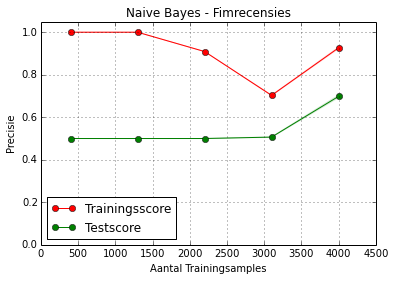
\includegraphics[width=5cm]{lc-movie-movie}}}%
    \label{fig:lc-movie-movie}
    \caption{Learning curve van de training van de Naive Bayes Classifier op filmrecensies}
\end{figure}

\begin{figure}[h!]
    \centering
    \subfloat{{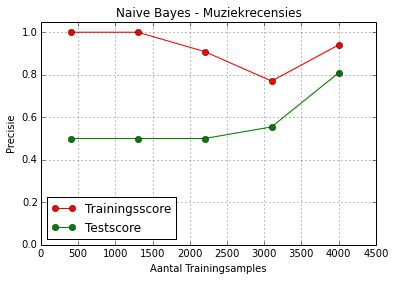
\includegraphics[width=5cm]{lc-music-music}}}%
    \label{fig:lc-music-music}
    \caption{Learning curve van de training van de Naive Bayes Classifier op muziekrecensies}
\end{figure}

\begin{figure}[h!]
    \centering
    \subfloat{{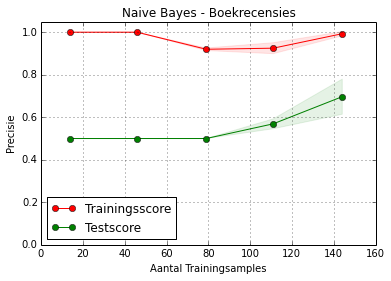
\includegraphics[width=5cm]{lc-boek-boek}}}%
    \label{fig:lc-boek-boek}
    \caption{Learning curve van de training van de Naive Bayes Classifier op boekrecensies}
\end{figure}

\section{Confusion matrixen}

\begin{table}[h]
\centering
\setlength\tabcolsep{4pt}
\begin{minipage}[t]{0.48\textwidth}
\centering
\begin{tabular}{lll}
                                 & \textbf{P}               & \textbf{N}               \\ \cline{2-3} 
\multicolumn{1}{l|}{\textbf{P'}} & \multicolumn{1}{l|}{824} & \multicolumn{1}{l|}{175} \\ \cline{2-3} 
\multicolumn{1}{l|}{\textbf{N'}} & \multicolumn{1}{l|}{410} & \multicolumn{1}{l|}{589} \\ \cline{2-3} 
\end{tabular}
\caption{Confusion matrix van de testset met filmrecensies door de  Naive Bayes Classifier, getraind op filmrecensies} 
\end{minipage}%
\hfill
\begin{minipage}[t]{0.48\textwidth}
\centering
\begin{tabular}{lll}
                                 & \textbf{P}               & \textbf{N}               \\ \cline{2-3} 
\multicolumn{1}{l|}{\textbf{P'}} & \multicolumn{1}{l|}{879} & \multicolumn{1}{l|}{120} \\ \cline{2-3} 
\multicolumn{1}{l|}{\textbf{N'}} & \multicolumn{1}{l|}{227} & \multicolumn{1}{l|}{772} \\ \cline{2-3} 
\end{tabular}
\caption{Confusion matrix van de testset met muziekrecensies door de  Naive Bayes Classifier, getraind op muziekrecensies} 
\end{minipage}
\end{table}

\begin{table}
\centering
\begin{tabular}{lll}
                                 & \textbf{P}               & \textbf{N}            \\ \cline{2-3} 
\multicolumn{1}{l|}{\textbf{P'}} & \multicolumn{1}{l|}{31} & \multicolumn{1}{l|}{5} \\ \cline{2-3} 
\multicolumn{1}{l|}{\textbf{N'}} & \multicolumn{1}{l|}{15} & \multicolumn{1}{l|}{21} \\ \cline{2-3} 
\end{tabular}
\caption{Confusion matrix van de testset met boekrecensies door de  Naive Bayes Classifier, getraind op boekrecensies} 
\end{table}
 

\begin{table}
\centering
\setlength\tabcolsep{4pt}
\begin{minipage}[t]{0.48\textwidth}
\centering
\begin{tabular}{lll}
                                 & \textbf{P}               & \textbf{N}               \\ \cline{2-3} 
\multicolumn{1}{l|}{\textbf{P'}} & \multicolumn{1}{l|}{655} & \multicolumn{1}{l|}{345} \\ \cline{2-3} 
\multicolumn{1}{l|}{\textbf{N'}} & \multicolumn{1}{l|}{413} & \multicolumn{1}{l|}{586} \\ \cline{2-3} 
\end{tabular}
\caption{Confusion matrix van de testset ,bestaande uit muziekrecensies, door de  Naive Bayes Classifier, getraind op filmrecensies}
\end{minipage}%
\hfill
\begin{minipage}[t]{0.48\textwidth}
\centering
\begin{tabular}{lll}
                                 & \textbf{P}               & \textbf{N}               \\ \cline{2-3} 
\multicolumn{1}{l|}{\textbf{P'}} & \multicolumn{1}{l|}{54} & \multicolumn{1}{l|}{18} \\ \cline{2-3} 
\multicolumn{1}{l|}{\textbf{N'}} & \multicolumn{1}{l|}{31} & \multicolumn{1}{l|}{41} \\ \cline{2-3} 
\end{tabular}
\caption{Confusion matrix van de testset, bestaande uit boekrecensies, door de  Naive Bayes Classifier, getraind op filmrecensies} 
\end{minipage}
\end{table}


\begin{table}
\centering
\setlength\tabcolsep{4pt}
\begin{minipage}[t]{0.48\textwidth}
\centering
\begin{tabular}{lll}
                                 & \textbf{P}               & \textbf{N}               \\ \cline{2-3} 
\multicolumn{1}{l|}{\textbf{P'}} & \multicolumn{1}{l|}{43} & \multicolumn{1}{l|}{29} \\ \cline{2-3} 
\multicolumn{1}{l|}{\textbf{N'}} & \multicolumn{1}{l|}{26} & \multicolumn{1}{l|}{46} \\ \cline{2-3} 
\end{tabular}
\caption{Confusion matrix van de testset, bestaande uit boekrecensies, door de  Naive Bayes Classifier, getraind op muziekrecensies} 
\end{minipage}%
\hfill
\begin{minipage}[t]{0.48\textwidth}
\centering
\begin{tabular}{lll}
                                 & \textbf{P}               & \textbf{N}               \\ \cline{2-3} 
\multicolumn{1}{l|}{\textbf{P'}} & \multicolumn{1}{l|}{691} & \multicolumn{1}{l|}{308} \\ \cline{2-3} 
\multicolumn{1}{l|}{\textbf{N'}} & \multicolumn{1}{l|}{469} & \multicolumn{1}{l|}{530} \\ \cline{2-3} 
\end{tabular}
\caption{Confusion matrix van de testset ,bestaande uit filmrecensies, door de  Naive Bayes Classifier, getraind op muziekrecensies} 
\end{minipage}
\end{table}

\begin{table}
\centering
\setlength\tabcolsep{4pt}
\begin{minipage}[t]{0.48\textwidth}
\centering
\begin{tabular}{lll}
                                 & \textbf{P}               & \textbf{N}               \\ \cline{2-3} 
\multicolumn{1}{l|}{\textbf{P'}} & \multicolumn{1}{l|}{604} & \multicolumn{1}{l|}{395} \\ \cline{2-3} 
\multicolumn{1}{l|}{\textbf{N'}} & \multicolumn{1}{l|}{475} & \multicolumn{1}{l|}{524} \\ \cline{2-3} 
\end{tabular}
\caption{Confusion matrix van de testset, bestaande uit muziekrecensies, door de  Naive Bayes Classifier, getraind op boekrecensies} 
\end{minipage}%
\hfill
\begin{minipage}[t]{0.48\textwidth}
\centering
\begin{tabular}{lll}
                                 & \textbf{P}               & \textbf{N}               \\ \cline{2-3} 
\multicolumn{1}{l|}{\textbf{P'}} & \multicolumn{1}{l|}{539} & \multicolumn{1}{l|}{460} \\ \cline{2-3} 
\multicolumn{1}{l|}{\textbf{N'}} & \multicolumn{1}{l|}{414} & \multicolumn{1}{l|}{585} \\ \cline{2-3} 
\end{tabular}
\caption{Confusion matrix van de testset ,bestaande uit filmrecensies, door de  Naive Bayes Classifier, getraind op boekrecensies} 
\end{minipage}
\end{table}


